\documentclass[12pt,a4paper]{article}

\usepackage[a4paper,margin=1in]{geometry}
\usepackage{newtxtext,newtxmath}
\usepackage{setspace}
\usepackage{graphicx}
\usepackage{booktabs}
\usepackage{longtable}
\usepackage{tabularx}
\usepackage{array}
\usepackage{enumitem}
\usepackage{tikz}
\usetikzlibrary{arrows.meta,positioning,shapes.geometric,fit}
\usepackage{hyperref}
\usepackage[numbers]{natbib}
\usepackage{fancyhdr}

\setstretch{1.2}
\setlength{\parindent}{0pt}
\setlength{\parskip}{6pt}
\hypersetup{colorlinks=true,linkcolor=black,citecolor=black,urlcolor=blue}

\pagestyle{fancy}
\fancyhf{}
\fancyfoot[C]{\thepage}
\renewcommand{\headrulewidth}{0pt}

\title{UniPlanner Repository Implementation Report \\ Structured Approach Analysis}
\author{Repository: kritikadangal1122-debug/finalyearproject-uniplanner}
\date{\today}

\begin{document}

\maketitle
\thispagestyle{fancy}

\tableofcontents
\newpage

\section{Structured Approach to Repository Scope and Execution Context}

\subsection{Structured Approach to Runtime Composition}

The repository runs as a Node.js modular monolith with Express as the active runtime entrypoint. The production entrypoint in package scripts is \texttt{node server/index.js}, not a Vite command, and the server listens on port \texttt{4000} by default \cite{repo-readme}. The server startup also attempts Cloudinary preset verification through \texttt{ensureUnsignedPreset()}, which is non-fatal when environment variables are not configured \cite{repo-server-app,repo-upload}.

\subsection{Structured Approach to Deliverable Boundaries}

Implementation in this repository is split across two UI tracks:
\begin{itemize}[leftmargin=1.5em]
  \item A static multi-page web interface under \texttt{public/} with modular JavaScript scripts for role-specific workflows.
  \item A React + TypeScript interface under \texttt{src/} that uses routing and context state management.
\end{itemize}

The active server serves \texttt{public/index.html} for non-API routes, which means the static web UI is directly integrated into the current backend execution path \cite{repo-server-app,repo-public-ui,repo-react-ui}.

\subsection{Structured Approach to Analysis Method}

This report is populated from direct repository inspection of backend modules, middleware, state persistence, frontend scripts, API wrappers, and migration scripts. The approach prioritizes implementation reality over aspirational architecture notes. For example, documentation files mention PostgreSQL and Redis, while executable code persists runtime state in a local JSON snapshot file under \texttt{server/data/learning-os.json} \cite{repo-store}.

\begin{table}[h]
\centering
\caption{Primary Executable Surfaces Identified}
\begin{tabularx}{\linewidth}{>{\raggedright\arraybackslash}p{3.0cm} >{\raggedright\arraybackslash}X >{\raggedright\arraybackslash}p{3.2cm}}
\toprule
Surface & Function in Current Implementation & Evidence \\
\midrule
\texttt{server/index.js} & Bootstraps API server and Cloudinary preset check & Runtime startup path \\
\texttt{server/app.js} & Composes middleware, registers domain modules, serves static assets & Express assembly \\
\texttt{server/modules/*.js} & Encapsulates API routes by domain context & API boundary layer \\
\texttt{public/*.html + public/js/*.js} & Role-based user workflows rendered as static pages & Active served UI \\
\texttt{src/*.tsx} & Alternative React client with richer component model & Secondary client track \\
\texttt{scripts/migrate-to-firebase.mjs} & Full snapshot migration into Firebase Realtime Database & Data export path \\
\bottomrule
\end{tabularx}
\end{table}

\begin{figure}[h]
\centering
\fbox{\parbox[c][2.2in][c]{0.92\linewidth}{\centering
Interface Figure Placeholder: Login and dashboard transition for the static \texttt{public/} UI, showing role-dependent navigation.
}}
\caption{Planned visual evidence slot for role-aware UI transition flow.}
\label{fig:ui-login-dashboard-placeholder}
\end{figure}

\section{Structured Approach to System Architecture and Module Topology}

\subsection{Structured Approach to Express Application Topology}

The Express app composes JSON body parsing, targeted CORS handling, API route registration, admin reset tooling, static upload serving, and SPA-like fallback routing for public assets \cite{repo-server-app,express-docs}. The API namespace is normalized through \texttt{API\_PREFIX = /api} inside shared HTTP helpers \cite{repo-security}.

\begin{figure}[h]
\centering
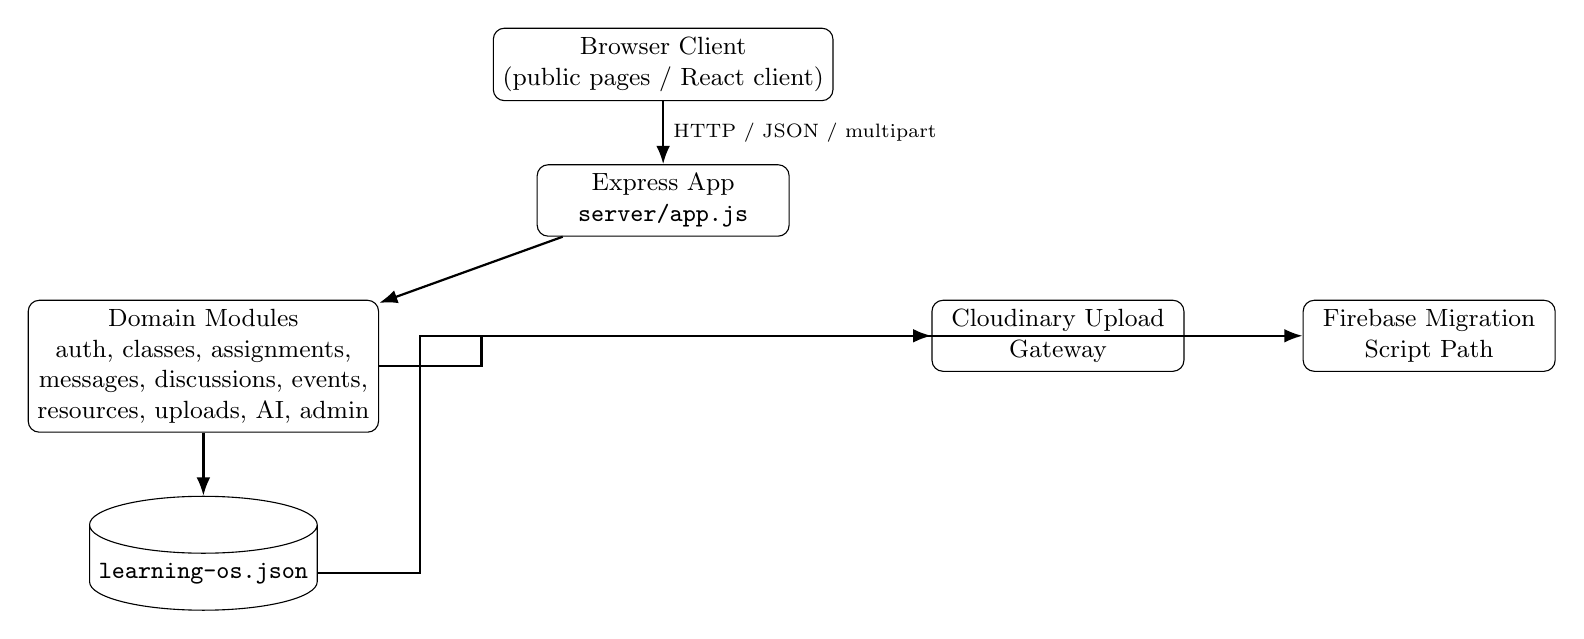
\begin{tikzpicture}[
  node distance=8mm and 10mm,
  box/.style={draw, rounded corners, align=center, minimum width=3.2cm, minimum height=0.9cm, font=\small},
  data/.style={draw, cylinder, shape border rotate=90, aspect=0.25, align=center, minimum height=1.0cm, minimum width=2.2cm, font=\small},
  arrow/.style={-Latex, thick}
]
\node[box] (client) {Browser Client\\(public pages / React client)};
\node[box, below=of client] (app) {Express App\\\texttt{server/app.js}};
\node[box, below left=of app, xshift=-10mm] (modules) {Domain Modules\\auth, classes, assignments,\\messages, discussions, events,\\resources, uploads, AI, admin};
\node[data, below=of modules] (jsondb) {\texttt{learning-os.json}};
\node[box, below right=of app, xshift=8mm] (cloudinary) {Cloudinary Upload\\Gateway};
\node[box, right=of cloudinary, xshift=5mm] (firebase) {Firebase Migration\\Script Path};

\draw[arrow] (client) -- node[right,font=\scriptsize]{HTTP / JSON / multipart} (app);
\draw[arrow] (app) -- (modules);
\draw[arrow] (modules) -- (jsondb);
\draw[arrow] (modules.east) -- ++(1.3,0) |- (cloudinary.west);
\draw[arrow] (jsondb.east) -- ++(1.3,0) |- (firebase.west);
\end{tikzpicture}
\caption{Repository-implemented architecture topology.}
\label{fig:architecture-topology}
\end{figure}

\subsection{Structured Approach to Backend Domain Boundaries}

\texttt{server/modules/index.js} registers 12 module groups in a deterministic order: authentication, admin, dashboard, classes, assignments, discussions, messages, notifications, events, resources, AI helpers, and upload handling \cite{repo-server-modules}. This achieves bounded routing concerns without introducing cross-process microservices.

\begin{table}[h]
\centering
\caption{Module Boundary and Core Responsibility Mapping}
\begin{tabularx}{\linewidth}{>{\raggedright\arraybackslash}p{3.2cm} >{\raggedright\arraybackslash}X >{\raggedright\arraybackslash}p{3.1cm}}
\toprule
Module & Core Responsibility & Access Pattern \\
\midrule
Auth & Health/meta endpoints, credential validation, session token issuance & Public + authenticated \\
Admin & User lifecycle and role management & Admin only \\
Dashboard & Snapshot access, widget preference updates, analytics overview & Authenticated \\
Classes & Class create/join/archive lifecycle & Role-gated write operations \\
Assignments & Assignment retrieval and creation & Teacher/admin create \\
Upload & Resource/submission file handling and grading updates & Mixed role controls \\
Notifications & Inbox fetch, mark-read mutation, SSE unread stream & Authenticated \\
AI & Summaries, quiz generation, feedback synthesis & Input-validated POST endpoints \\
\bottomrule
\end{tabularx}
\end{table}

\subsection{Structured Approach to Architecture Reality Check}

Architecture documentation files describe a planned stack using PostgreSQL, Redis, and S3-compatible storage. Current executable code persists state in JSON files and uses Cloudinary for file object storage. Therefore, the implemented architecture is best classified as a local-file-backed modular monolith with optional cloud upload and optional Firebase migration utilities, rather than a distributed data platform \cite{repo-store,repo-upload,firebase-admin-docs}.

\section{Structured Approach to Backend API and Middleware Implementation}

\subsection{Structured Approach to Middleware Pipeline}

Backend request handling follows this sequence:
\begin{enumerate}[leftmargin=1.5em]
  \item Express JSON parser with 5 MB body limit.
  \item CORS allowlist middleware for local Live Server origins.
  \item Route-level handlers composed using \texttt{createJsonRoute} to normalize exception handling.
  \item Auth guards through \texttt{requireAuth} and role checks through \texttt{requireRole}.
  \item Global error fallback returning a 500 JSON payload.
\end{enumerate}

This pipeline standardizes error shape and reduces repetitive try/catch blocks in module files \cite{repo-server-app,repo-security}.

\subsection{Structured Approach to Endpoint Inventory}

\begin{longtable}{>{\raggedright\arraybackslash}p{2.4cm} >{\raggedright\arraybackslash}p{1.7cm} >{\raggedright\arraybackslash}p{7.8cm}}
\caption{Implemented API Endpoint Inventory by Capability}\\
\toprule
Path & Method & Implemented Behavior \\
\midrule
\endfirsthead
\toprule
Path & Method & Implemented Behavior \\
\midrule
\endhead
\texttt{/api/health} & GET & Returns service heartbeat and configuration flag details. \\
\texttt{/api/meta} & GET & Returns module/capability metadata payload. \\
\texttt{/api/auth/login} & POST & Validates email/password hash and issues signed JWT plus server-side session. \\
\texttt{/api/auth/me} & GET & Returns current user and stored permissions for active session token. \\
\texttt{/api/state} & GET/PUT & Reads and replaces public app snapshot state. \\
\texttt{/api/preferences/widget-order} & PUT & Updates dashboard widget order in preferences. \\
\texttt{/api/analytics/overview} & GET & Returns role analytics, health signals, and next-best-action recommendation. \\
\texttt{/api/insights/next-best-action/:userId} & GET & Returns recommendation with self-or-admin visibility constraints. \\
\texttt{/api/classes} & GET/POST & Lists classes and creates classes for teacher/admin roles. \\
\texttt{/api/classes/join} & POST & Enrolls user by class code and increments class student count. \\
\texttt{/api/classes/:classId/archive} & POST & Archives class with ownership check for teacher role. \\
\texttt{/api/assignments} & GET/POST & Lists assignments and creates assignment definitions. \\
\texttt{/api/discussions/:classId} & GET & Fetches class-specific thread list. \\
\texttt{/api/discussions} & POST & Creates thread and records discussion analytics event. \\
\texttt{/api/messages/:classId} & GET & Fetches class-scoped chat timeline. \\
\texttt{/api/messages} & POST & Writes class chat message to snapshot. \\
\texttt{/api/notifications} & GET & Returns notification list from snapshot. \\
\texttt{/api/notifications/:id/read} & PATCH & Marks a single notification as read. \\
\texttt{/api/notifications/stream} & GET & Streams unread notification count every 15 seconds with SSE. \\
\texttt{/api/events} & GET/POST & Lists and creates calendar events with role checks. \\
\texttt{/api/resources} & GET/POST & Lists and creates resource metadata objects. \\
\texttt{/api/upload/resource} & POST & Uploads teacher/admin file to Cloudinary and records resource object. \\
\texttt{/api/upload/submission} & POST & Uploads student submission file and links to assignment. \\
\texttt{/api/submissions/:id} & DELETE & Deletes own submission and decrements assignment submission count. \\
\texttt{/api/submissions/:id/grade} & PATCH & Updates score/feedback and recalculates assignment average score. \\
\texttt{/api/ai/study-copilot/summary} & POST & Heuristic text summary and key points generation. \\
\texttt{/api/ai/study-copilot/quiz} & POST & Deterministic question generation from source text. \\
\texttt{/api/ai/assignment-feedback} & POST & Feedback synthesis based on word-count and rubric focus. \\
\texttt{/api/ai/discussion-summary} & POST & Discussion summarization and action item synthesis. \\
\texttt{/api/admin/users} & GET/POST & Lists and creates users (admin only). \\
\texttt{/api/admin/users/:userId} & PUT/DELETE & Updates or deletes user with last-admin guard. \\
\texttt{/api/admin/users/:userId/role} & PATCH & Changes user role with validation. \\
\bottomrule
\end{longtable}

\subsection{Structured Approach to AI Assist Features}

AI endpoints in \texttt{server/ai.js} are deterministic prompt-free utilities, not remote LLM calls. The summarization and quiz logic derives output from sentence segmentation and keyword extraction. Assignment feedback score uses word count heuristics bounded between 40 and 98. This gives predictable behavior for offline or low-dependency operation while preserving AI-like interaction affordances in UI workflows \cite{repo-server-modules}.

\begin{figure}[h]
\centering
\fbox{\parbox[c][2.1in][c]{0.92\linewidth}{\centering
Backend API Figure Placeholder: Endpoint call trace with request payload, auth header validation step, and JSON snapshot mutation outcome.
}}
\caption{Planned trace visualization for API request lifecycle evidence.}
\label{fig:api-trace-placeholder}
\end{figure}

\section{Structured Approach to Frontend Integration and User Workflows}

\subsection{Structured Approach to Static Multi-Page Web Client}

The static client under \texttt{public/} drives user-facing workflows through modular scripts:\
\texttt{app.js} handles layout shell, role-based navigation, notification panel behavior, and guard redirects;\
\texttt{store.js} holds local state transitions and persistence;\
\texttt{cloudinary.js} supports direct browser-to-Cloudinary uploads;\
\texttt{api.js} wraps backend calls with bearer headers \cite{repo-public-ui,repo-upload}.

Role-specific pages include dashboard, classes, class detail, assignments, grading, collaboration, analytics, calendar, resources, settings, and admin management.

\subsection{Structured Approach to React Client Track}

The repository also contains a React + TypeScript application with route-guarded paths (\texttt{/app}, \texttt{/app/classes}, \texttt{/app/assignments}, \texttt{/app/grading}, etc.) and context-driven state operations \cite{repo-react-ui}. This client calls the same backend API wrapper for login, analytics, uploads, and grading actions.

The two client tracks currently coexist. Static pages are directly served by Express, while React code remains a separate runtime path that would require Vite execution. This dual-track structure is important for release planning because feature drift can occur when business logic exists in both \texttt{public/js/store.js} and \texttt{src/context/LmsContext.tsx}.

\subsection{Structured Approach to Workflow Coverage by Role}

\begin{table}[h]
\centering
\caption{Implemented Workflow Coverage by Role}
\begin{tabularx}{\linewidth}{>{\raggedright\arraybackslash}p{2.0cm} >{\raggedright\arraybackslash}X >{\raggedright\arraybackslash}X}
\toprule
Role & Primary UI Workflows & Primary Backend Dependencies \\
\midrule
Student & Login, join class, submit assignment, follow discussions, view analytics and notifications & \texttt{/auth/login}, \texttt{/classes/join}, \texttt{/upload/submission}, \texttt{/discussions}, \texttt{/notifications} \\
Teacher & Create classes, create assignments, upload resources, grade submissions, track class analytics & \texttt{/classes}, \texttt{/assignments}, \texttt{/upload/resource}, \texttt{/submissions/:id/grade}, \texttt{/analytics/overview} \\
Admin & User provisioning, role updates, platform-level analytics review, reset demo state & \texttt{/admin/users*}, \texttt{/insights/next-best-action/:id}, \texttt{/admin/reset-demo} \\
\bottomrule
\end{tabularx}
\end{table}

\begin{figure}[h]
\centering
\fbox{\parbox[c][2.2in][c]{0.92\linewidth}{\centering
UI Workflow Placeholder: Student submission path from assignments page to Cloudinary upload and server submission record creation.
}}
\caption{Planned capture slot for assignment submission workflow in the static UI.}
\label{fig:student-submission-ui-placeholder}
\end{figure}

\section{Structured Approach to Data Persistence, Authentication, and Operational Workflows}

\subsection{Structured Approach to Snapshot-Centric Data Persistence}

The primary data store is a JSON file at \texttt{server/data/learning-os.json}. \texttt{LearningStore} initializes default state from seeded data, persists updates synchronously, and exposes helper methods for sessions, analytics events, submissions, and entity lookups \cite{repo-store}. This approach simplifies local development and demo reproducibility.

The persisted snapshot includes:
\begin{itemize}[leftmargin=1.5em]
  \item \texttt{app}: users, classes, assignments, discussions, messages, notifications, events, resources.
  \item \texttt{submissions}: uploaded student work records with grading metadata.
  \item \texttt{analyticsEvents}: append-only event feed used for dashboard signals.
  \item \texttt{sessions}: active token registry used for session revocation and expiry checks.
  \item \texttt{goals} and \texttt{permissions}: role and intervention signal support.
\end{itemize}

\subsection{Structured Approach to Authentication and Session Lifecycle}

Authentication combines JWT signing with server-side session storage:
\begin{enumerate}[leftmargin=1.5em]
  \item User credentials are validated by SHA-256 password hash comparison.
  \item JWT payload includes \texttt{sub}, \texttt{role}, \texttt{iat}, \texttt{exp}, and \texttt{jti}.
  \item Token is signed with HMAC-SHA256 using \texttt{LEARNING\_OS\_JWT\_SECRET}.
  \item Session record is stored in snapshot with expiration timestamp.
  \item \texttt{requireAuth} validates bearer token, signature, expiry, session presence, and user existence.
\end{enumerate}

This design adds revocation control compared with stateless JWT-only validation \cite{repo-security,node-crypto-docs}.

\begin{figure}[h]
\centering
\begin{tikzpicture}[
  node distance=7mm and 10mm,
  step/.style={draw, rounded corners, align=center, minimum width=3.2cm, minimum height=0.85cm, font=\small},
  arrow/.style={-Latex, thick}
]
\node[step] (u1) {Client submits\\email + password};
\node[step, right=of u1] (s1) {\texttt{/api/auth/login}\\hash + compare};
\node[step, right=of s1] (s2) {Sign JWT\\HMAC-SHA256};
\node[step, below=of s2] (s3) {Persist session\\in snapshot};
\node[step, left=of s3] (u2) {Client stores token\\Bearer header};
\node[step, left=of u2] (s4) {\texttt{requireAuth} verifies\\token + session + user};

\draw[arrow] (u1) -- (s1);
\draw[arrow] (s1) -- (s2);
\draw[arrow] (s2) -- (s3);
\draw[arrow] (s3) -- (u2);
\draw[arrow] (u2) -- (s4);
\end{tikzpicture}
\caption{Authentication and guarded request sequence implemented in the repository.}
\label{fig:auth-sequence}
\end{figure}

\subsection{Structured Approach to File Upload and Grading Workflow}

Resource and submission uploads use \texttt{multer.memoryStorage()} and forward file buffers to Cloudinary. The workflow enforces role constraints for resource upload and ownership constraints for submission deletion. Grading mutations update both submission records and assignment-level aggregate metrics (average score and status transition to graded) \cite{repo-upload,multer-docs,cloudinary-docs}.

\subsection{Structured Approach to Migration Workflow}

The repository includes \texttt{scripts/migrate-to-firebase.mjs} for full snapshot export to Firebase Realtime Database under \texttt{/learning\_os}. The migration script loads environment variables from \texttt{.env} and \texttt{.env.local}, sanitizes undefined values, computes entity counts, and uploads both metadata and full data payload using Firebase Admin SDK credentials \cite{firebase-admin-docs}.

\section{Structured Approach to Quality, Security, and Implementation Gaps}

\subsection{Structured Approach to Security Controls Present in Code}

Implemented controls include:
\begin{itemize}[leftmargin=1.5em]
  \item Timing-safe JWT signature verification using \texttt{timingSafeEqual}.
  \item Role-gated route mutations for admin, teacher, and student boundaries.
  \item Session expiry enforcement in addition to JWT expiry.
  \item Removal of password hash from outbound user payload through \texttt{toPublicUser} projection.
  \item Non-fatal startup behavior when cloud credentials are missing.
\end{itemize}

These controls provide practical baseline hardening for a demo-ready educational platform backend \cite{repo-security,repo-server-modules}.

\subsection{Structured Approach to Key Implementation Gaps Observed}

Repository analysis identifies several concrete gaps:
\begin{enumerate}[leftmargin=1.5em]
  \item \textbf{State model divergence}: static UI and React UI each implement overlapping state and workflow logic, increasing inconsistency risk.
  \item \textbf{Documentation-runtime mismatch}: docs mention PostgreSQL/Redis-style architecture while runtime persists JSON snapshots.
  \item \textbf{Client type mismatch risk}: \texttt{src/lib/api.ts} health typing does not fully align with backend \texttt{buildPlatformHealth} payload fields.
  \item \textbf{No automated test/lint scripts}: package scripts only expose \texttt{start}, \texttt{dev}, and migration command, limiting CI-style regression gates.
\end{enumerate}

\subsection{Structured Approach to Reliability and Maintainability Priorities}

A practical sequencing strategy derived from current implementation is:
\begin{enumerate}[leftmargin=1.5em]
  \item Consolidate to one frontend execution track per release branch.
  \item Introduce API contract tests around auth, classes, assignments, upload, and grading endpoints.
  \item Introduce schema validation at route boundaries for body/query payloads.
  \item Replace synchronous JSON writes with transaction-safe data persistence in a managed database when moving beyond single-instance deployment.
\end{enumerate}

\begin{figure}[h]
\centering
\fbox{\parbox[c][2.1in][c]{0.92\linewidth}{\centering
Reliability Evidence Placeholder: Comparative chart of API response consistency before and after endpoint contract validation.
}}
\caption{Planned measurement placeholder for reliability hardening progress.}
\label{fig:reliability-placeholder}
\end{figure}

\section{Structured Approach to Conclusion and Repository Readiness}

\subsection{Structured Approach to Current Readiness}

The repository already implements a cohesive educational workflow covering authentication, role-aware dashboards, classes, assignments, discussions, messaging, notifications, analytics summaries, uploads, AI-assisted feedback, and admin operations. The backend modules are cleanly segmented and exposed through a consistent API envelope, while frontend pages provide clear role-targeted UX paths \cite{repo-server-modules,repo-public-ui}.

\subsection{Structured Approach to Deployment Interpretation}

From implementation evidence, UniPlanner should currently be interpreted as a local-first monolith suitable for demo deployments and structured pilot environments. It includes extension hooks for Cloudinary object storage and Firebase snapshot migration, which are useful transition bridges toward managed infrastructure without immediate architectural overhaul \cite{repo-upload,firebase-admin-docs}.

\subsection{Structured Approach to Immediate Next Engineering Milestones}

The highest-value next milestones are to unify frontend logic, formalize API contract testing, and align documentation with executable architecture. Completing those steps will reduce drift, improve release confidence, and make later transitions to relational persistence and distributed components predictable and lower risk.


\bibliographystyle{IEEEtran}
\bibliography{references}

\end{document}
